\clearpage\SourceLeaf{291}

Man kann die möglichen Tracte auch als geschlossene ansehen, und folglich
aus jedem möglichen durch Vorrückung des Anfangsgliedes andere ableiten.
Die 24 möglichen, welche sich unter den 105 Tracten für 4 vollständige
Knoten befinden, erscheinen in dieser Abhängigkeit so:

\begin{center}
\begin{tabular}{l@{\qquad}l}
1.\quad 39 & I.\ 4 \quad IV.\ 1 \quad VIII.\ 1 \\
54.\quad 89 & II.\ 2 \quad III.\ 4 \\
15.\ 105.\ 73.\ 33 & II.\ 5 \\
3.\ 45.\ 7.\ 75.\ 31.\ 9.\ 81.\ 37 & \\
10.\ 91.\ 46.\ 48.\ 56.\ 100.\ 76.\ 40 & \\
\end{tabular}
\end{center}

\begin{center}
\resizebox{1.6875cm}{!}{%
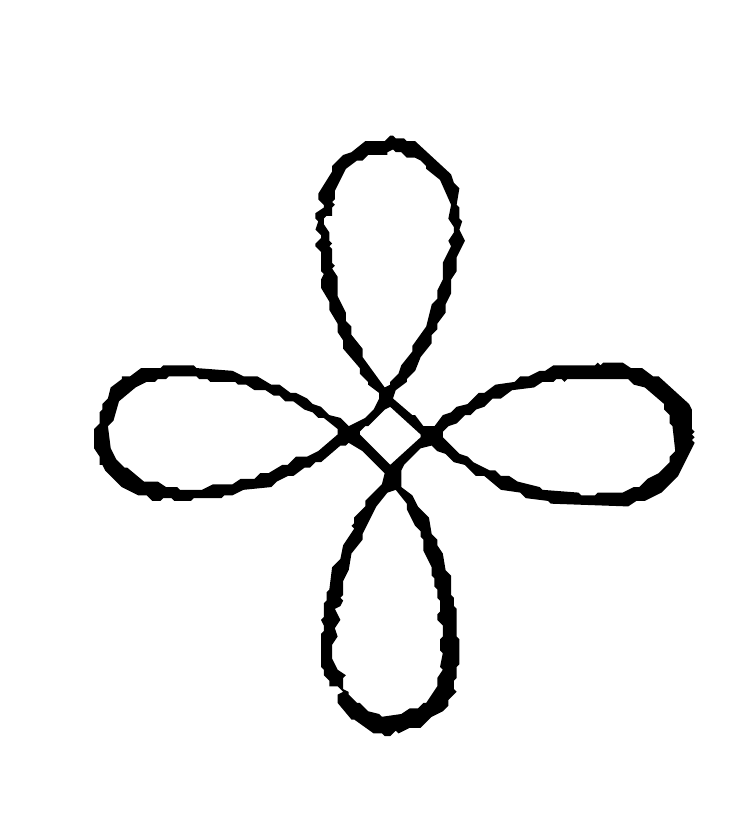
\begin{tikzpicture}[x=1pt,y=-1pt]
\path[use as bounding box] (0,0) rectangle (250,278);
\path[fill=black,draw=none,even odd rule]
(132,39) -- (131,39) -- (129,41) -- (122,41) -- (117,45) -- (114,46) -- (110,50) -- (110,52) -- (105,60) -- (105,62) -- (107,64) -- (107,65) -- (104,67) -- (104,69) -- (105,70) -- (104,73) -- (106,75) -- (106,76) -- (104,78) -- (104,79) -- (106,81) -- (106,88) -- (107,89) -- (106,91) -- (106,94) -- (109,99) -- (109,102) -- (112,107) -- (112,110) -- (114,113) -- (114,116) -- (120,123) -- (120,125) -- (123,128) -- (123,129) -- (127,132) -- (127,134) -- (125,138) -- (122,141) -- (116,144) -- (113,141) -- (109,140) -- (106,137) -- (103,136) -- (101,134) -- (97,132) -- (95,132) -- (91,129) -- (88,129) -- (83,126) -- (78,126) -- (74,124) -- (61,123) -- (60,122) -- (49,122) -- (48,123) -- (41,123) -- (37,126) -- (34,126) -- (34,127) -- (30,130) -- (29,134) -- (27,136) -- (27,138) -- (26,139) -- (26,143) -- (24,145) -- (24,152) -- (26,155) -- (26,158) -- (27,158) -- (28,160) -- (34,166) -- (40,169) -- (43,169) -- (45,171) -- (48,171) -- (49,170) -- (52,170) -- (53,171) -- (59,171) -- (60,170) -- (70,170) -- (71,169) -- (74,169) -- (78,167) -- (88,166) -- (90,164) -- (94,162) -- (96,162) -- (100,159) -- (102,159) -- (104,157) -- (106,157) -- (113,151) -- (115,151) -- (116,150) -- (121,153) -- (129,161) -- (128,165) -- (122,171) -- (122,173) -- (118,177) -- (118,179) -- (117,180) -- (118,181) -- (114,187) -- (113,192) -- (110,195) -- (109,203) -- (108,204) -- (108,207) -- (107,208) -- (107,213) -- (106,214) -- (107,216) -- (107,218) -- (106,219) -- (106,231) -- (107,232) -- (107,234) -- (109,236) -- (109,238) -- (112,238) -- (114,240) -- (112,241) -- (112,244) -- (117,250) -- (118,250) -- (125,255) -- (128,255) -- (129,256) -- (131,256) -- (133,254) -- (134,255) -- (138,253) -- (142,253) -- (146,249) -- (150,247) -- (152,245) -- (152,243) -- (155,240) -- (154,239) -- (154,236) -- (155,235) -- (155,231) -- (156,230) -- (156,221) -- (155,220) -- (155,210) -- (154,209) -- (154,206) -- (153,205) -- (153,198) -- (151,196) -- (150,190) -- (148,187) -- (148,185) -- (146,183) -- (145,177) -- (141,173) -- (139,169) -- (135,166) -- (135,160) -- (136,158) -- (142,152) -- (146,151) -- (148,153) -- (151,154) -- (154,157) -- (158,158) -- (162,162) -- (165,162) -- (171,167) -- (178,168) -- (180,170) -- (188,171) -- (189,172) -- (217,173) -- (220,171) -- (223,171) -- (229,168) -- (235,162) -- (241,150) -- (240,149) -- (241,148) -- (240,147) -- (241,146) -- (240,145) -- (240,138) -- (239,136) -- (228,126) -- (226,126) -- (222,123) -- (218,123) -- (215,121) -- (208,121) -- (207,122) -- (206,121) -- (205,122) -- (190,122) -- (187,124) -- (185,124) -- (181,126) -- (178,126) -- (176,128) -- (169,129) -- (165,132) -- (163,132) -- (159,136) -- (155,137) -- (153,139) -- (150,140) -- (147,144) -- (143,144) -- (140,140) -- (139,140) -- (132,134) -- (133,131) -- (137,128) -- (137,127) -- (140,124) -- (142,119) -- (146,114) -- (146,111) -- (148,109) -- (148,107) -- (151,103) -- (151,100) -- (153,96) -- (153,91) -- (155,88) -- (155,83) -- (158,77) -- (156,73) -- (157,70) -- (156,69) -- (156,65) -- (155,64) -- (156,58) -- (154,56) -- (153,53) -- (140,41) -- (137,41) -- (136,40) -- (133,40) -- cycle
(133,167) -- (137,172) -- (137,174) -- (140,180) -- (142,182) -- (142,184) -- (143,185) -- (143,189) -- (146,195) -- (146,198) -- (147,199) -- (147,202) -- (148,203) -- (148,206) -- (149,207) -- (149,211) -- (148,212) -- (148,214) -- (150,216) -- (150,220) -- (149,221) -- (149,225) -- (150,226) -- (149,231) -- (150,232) -- (148,235) -- (148,238) -- (144,244) -- (143,244) -- (141,246) -- (138,246) -- (135,248) -- (128,249) -- (127,248) -- (123,247) -- (120,244) -- (119,244) -- (116,241) -- (116,240) -- (114,239) -- (114,235) -- (115,234) -- (112,232) -- (110,228) -- (110,223) -- (112,220) -- (111,217) -- (113,214) -- (111,210) -- (113,209) -- (114,207) -- (113,206) -- (114,205) -- (114,200) -- (116,196) -- (117,190) -- (121,185) -- (121,183) -- (126,173) -- (130,168) -- cycle
(131,137) -- (142,147) -- (142,148) -- (131,158) -- (120,147) -- (120,146) -- (122,144) -- (123,144) -- (129,138) -- cycle
(150,146) -- (152,144) -- (155,143) -- (158,140) -- (160,140) -- (162,138) -- (165,137) -- (168,134) -- (171,134) -- (175,131) -- (183,130) -- (186,128) -- (190,128) -- (191,127) -- (193,127) -- (194,128) -- (195,127) -- (217,127) -- (219,129) -- (223,130) -- (230,136) -- (230,138) -- (232,140) -- (232,143) -- (233,144) -- (234,153) -- (232,155) -- (232,157) -- (228,161) -- (224,163) -- (221,166) -- (219,166) -- (215,168) -- (206,168) -- (205,169) -- (200,169) -- (199,168) -- (186,167) -- (185,166) -- (177,164) -- (174,162) -- (171,162) -- (169,160) -- (167,160) -- (161,157) -- (159,155) -- (156,154) -- (150,148) -- cycle
(29,144) -- (31,142) -- (33,135) -- (39,130) -- (43,128) -- (46,128) -- (47,127) -- (50,127) -- (51,126) -- (61,126) -- (62,127) -- (65,127) -- (66,128) -- (75,128) -- (76,129) -- (79,129) -- (82,131) -- (86,131) -- (89,133) -- (91,133) -- (93,135) -- (96,135) -- (100,138) -- (103,139) -- (105,141) -- (107,141) -- (112,145) -- (112,147) -- (105,153) -- (101,155) -- (97,155) -- (94,158) -- (92,158) -- (87,161) -- (84,161) -- (82,163) -- (77,163) -- (74,165) -- (67,165) -- (63,167) -- (55,167) -- (54,166) -- (50,166) -- (47,164) -- (42,164) -- (36,159) -- (35,159) -- (32,156) -- (30,152) -- cycle
(132,44) -- (133,45) -- (135,45) -- (137,47) -- (140,47) -- (142,48) -- (144,50) -- (144,51) -- (149,55) -- (153,64) -- (152,69) -- (154,72) -- (154,74) -- (152,77) -- (153,79) -- (150,85) -- (150,91) -- (148,95) -- (148,98) -- (146,100) -- (144,108) -- (139,115) -- (139,117) -- (135,122) -- (134,125) -- (131,128) -- (131,129) -- (129,130) -- (121,119) -- (121,116) -- (117,111) -- (117,108) -- (115,106) -- (115,103) -- (112,97) -- (112,90) -- (110,87) -- (111,86) -- (110,85) -- (110,80) -- (109,79) -- (110,78) -- (109,77) -- (109,74) -- (107,71) -- (107,69) -- (108,68) -- (110,68) -- (110,65) -- (111,64) -- (110,63) -- (111,62) -- (111,59) -- (115,51) -- (119,48) -- (121,48) -- (123,46) -- (130,46) -- (130,45) -- cycle;
\end{tikzpicture}%
}
\hspace{.5em}\resizebox{1.575cm}{!}{%
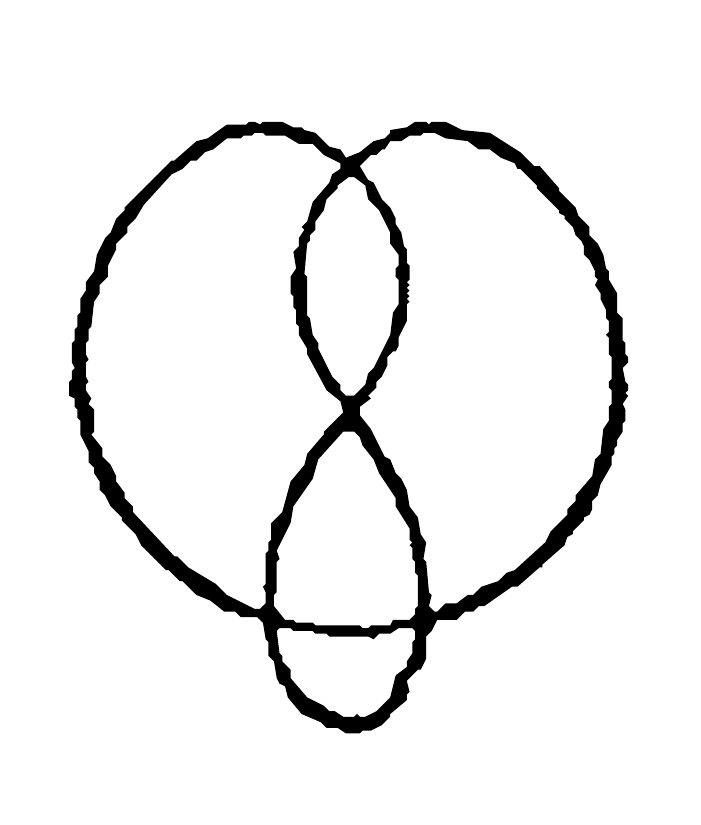
\begin{tikzpicture}[x=1pt,y=-1pt]
\path[use as bounding box] (0,0) rectangle (233,278);
\path[fill=black,draw=none,even odd rule]
(72,35) -- (65,40) -- (61,41) -- (53,48) -- (52,48) -- (35,65) -- (35,66) -- (32,69) -- (30,74) -- (28,76) -- (25,82) -- (24,88) -- (21,92) -- (21,95) -- (19,98) -- (19,103) -- (18,104) -- (18,108) -- (17,109) -- (17,113) -- (16,114) -- (16,121) -- (17,123) -- (16,124) -- (16,127) -- (15,128) -- (15,133) -- (17,134) -- (17,137) -- (18,138) -- (18,141) -- (19,142) -- (19,147) -- (22,153) -- (22,157) -- (24,159) -- (24,161) -- (26,164) -- (26,167) -- (28,169) -- (30,173) -- (34,177) -- (34,178) -- (39,183) -- (41,187) -- (50,196) -- (51,196) -- (55,200) -- (56,200) -- (61,205) -- (66,207) -- (71,211) -- (75,211) -- (77,213) -- (83,213) -- (85,215) -- (86,221) -- (87,222) -- (87,227) -- (89,229) -- (90,235) -- (91,237) -- (93,238) -- (94,242) -- (99,248) -- (106,251) -- (108,253) -- (112,253) -- (115,255) -- (120,255) -- (121,254) -- (124,254) -- (128,252) -- (131,249) -- (131,248) -- (137,243) -- (137,241) -- (138,240) -- (137,236) -- (141,232) -- (142,232) -- (144,228) -- (144,220) -- (146,218) -- (148,214) -- (155,214) -- (158,211) -- (161,211) -- (163,209) -- (165,209) -- (175,202) -- (177,202) -- (185,195) -- (186,195) -- (186,194) -- (194,187) -- (195,184) -- (197,183) -- (197,182) -- (201,178) -- (201,177) -- (203,176) -- (204,174) -- (204,171) -- (206,169) -- (207,165) -- (211,158) -- (211,155) -- (212,154) -- (212,152) -- (213,151) -- (213,149) -- (215,146) -- (215,143) -- (216,142) -- (216,138) -- (215,136) -- (217,133) -- (216,132) -- (217,131) -- (217,129) -- (216,128) -- (215,123) -- (217,121) -- (217,119) -- (216,118) -- (216,114) -- (215,113) -- (215,105) -- (213,103) -- (213,96) -- (210,91) -- (210,88) -- (209,87) -- (208,82) -- (206,78) -- (203,75) -- (203,72) -- (199,68) -- (198,65) -- (192,59) -- (192,58) -- (185,50) -- (183,50) -- (178,45) -- (167,38) -- (157,37) -- (151,34) -- (146,34) -- (145,35) -- (144,34) -- (140,34) -- (137,36) -- (131,37) -- (131,38) -- (129,40) -- (125,41) -- (120,45) -- (115,47) -- (113,44) -- (109,43) -- (104,38) -- (100,37) -- (99,36) -- (96,36) -- (92,34) -- (85,34) -- (84,35) -- (82,34) -- (80,34) -- (79,35) -- cycle
(90,218) -- (91,217) -- (95,217) -- (96,218) -- (103,218) -- (104,219) -- (108,219) -- (109,220) -- (123,220) -- (125,221) -- (127,219) -- (131,219) -- (134,217) -- (139,217) -- (140,218) -- (140,221) -- (139,222) -- (139,226) -- (137,229) -- (137,231) -- (133,234) -- (131,242) -- (126,247) -- (122,249) -- (120,249) -- (119,248) -- (118,249) -- (114,249) -- (111,247) -- (109,247) -- (107,245) -- (101,242) -- (95,235) -- (95,232) -- (92,229) -- (92,227) -- (91,226) -- cycle
(114,146) -- (118,146) -- (120,148) -- (121,151) -- (125,156) -- (127,161) -- (133,170) -- (133,173) -- (138,181) -- (138,185) -- (139,186) -- (138,187) -- (139,188) -- (139,192) -- (140,193) -- (140,197) -- (141,198) -- (141,209) -- (140,210) -- (140,212) -- (138,214) -- (132,214) -- (131,216) -- (124,216) -- (123,217) -- (121,217) -- (120,216) -- (104,216) -- (103,215) -- (97,215) -- (96,214) -- (93,214) -- (89,209) -- (89,205) -- (90,204) -- (90,193) -- (91,192) -- (90,189) -- (95,179) -- (96,173) -- (103,163) -- (105,156) -- cycle
(116,54) -- (118,54) -- (122,57) -- (123,62) -- (127,66) -- (131,74) -- (131,78) -- (134,82) -- (134,86) -- (133,87) -- (133,90) -- (134,91) -- (134,100) -- (132,103) -- (131,111) -- (125,123) -- (123,125) -- (122,129) -- (118,133) -- (115,133) -- (113,131) -- (113,129) -- (110,126) -- (105,116) -- (105,114) -- (103,111) -- (102,105) -- (101,104) -- (101,90) -- (100,89) -- (101,78) -- (102,77) -- (102,75) -- (104,73) -- (104,70) -- (107,66) -- (108,62) -- (112,58) -- (112,57) -- cycle
(143,38) -- (147,38) -- (151,40) -- (159,41) -- (163,44) -- (167,44) -- (171,47) -- (176,49) -- (177,51) -- (178,51) -- (184,57) -- (184,58) -- (192,66) -- (192,67) -- (194,68) -- (194,69) -- (197,72) -- (198,75) -- (200,77) -- (201,79) -- (201,82) -- (203,84) -- (205,88) -- (205,90) -- (206,91) -- (205,93) -- (207,96) -- (207,98) -- (209,102) -- (209,105) -- (210,106) -- (210,110) -- (209,111) -- (210,112) -- (210,118) -- (211,119) -- (211,127) -- (210,128) -- (210,130) -- (211,131) -- (211,136) -- (210,137) -- (210,142) -- (208,145) -- (207,154) -- (205,156) -- (204,162) -- (198,169) -- (198,171) -- (195,174) -- (195,176) -- (189,182) -- (187,186) -- (176,196) -- (173,197) -- (170,200) -- (164,202) -- (161,205) -- (159,205) -- (155,208) -- (151,208) -- (148,211) -- (147,211) -- (145,209) -- (146,205) -- (145,204) -- (144,193) -- (143,192) -- (144,186) -- (142,183) -- (141,177) -- (138,173) -- (137,167) -- (135,163) -- (133,161) -- (131,156) -- (129,155) -- (124,145) -- (120,140) -- (120,137) -- (124,134) -- (123,133) -- (126,130) -- (126,128) -- (128,126) -- (130,122) -- (130,119) -- (132,117) -- (133,117) -- (134,115) -- (134,112) -- (137,106) -- (137,100) -- (138,99) -- (137,98) -- (138,97) -- (137,96) -- (138,95) -- (137,94) -- (138,93) -- (137,92) -- (138,91) -- (138,86) -- (137,85) -- (137,80) -- (136,79) -- (135,74) -- (133,71) -- (133,69) -- (131,65) -- (128,62) -- (125,56) -- (123,55) -- (120,50) -- (124,46) -- (126,46) -- (128,44) -- (129,44) -- (131,41) -- (135,41) -- (138,39) -- (142,39) -- cycle
(82,38) -- (85,38) -- (86,39) -- (93,39) -- (98,42) -- (103,42) -- (107,46) -- (113,49) -- (113,51) -- (110,53) -- (109,56) -- (103,63) -- (101,70) -- (99,72) -- (100,73) -- (98,76) -- (98,79) -- (96,81) -- (97,87) -- (95,90) -- (95,96) -- (96,97) -- (96,101) -- (97,102) -- (97,107) -- (98,108) -- (98,111) -- (101,116) -- (101,118) -- (108,131) -- (113,135) -- (114,139) -- (107,146) -- (107,147) -- (101,154) -- (100,158) -- (95,164) -- (92,175) -- (88,179) -- (88,185) -- (87,186) -- (87,189) -- (86,190) -- (86,201) -- (85,202) -- (86,204) -- (86,208) -- (84,210) -- (82,210) -- (72,205) -- (68,201) -- (58,195) -- (54,191) -- (53,191) -- (38,175) -- (38,173) -- (35,170) -- (35,168) -- (32,164) -- (32,162) -- (30,158) -- (27,155) -- (27,152) -- (23,147) -- (24,146) -- (24,138) -- (22,136) -- (23,134) -- (21,131) -- (21,129) -- (22,128) -- (21,126) -- (21,121) -- (22,120) -- (21,118) -- (21,114) -- (22,113) -- (22,109) -- (23,108) -- (24,99) -- (26,96) -- (26,93) -- (29,90) -- (29,86) -- (32,80) -- (32,78) -- (36,74) -- (36,72) -- (39,69) -- (42,64) -- (52,53) -- (56,51) -- (59,48) -- (61,48) -- (64,45) -- (67,44) -- (72,40) -- (77,40) -- (78,39) -- (81,39) -- cycle;
\end{tikzpicture}%
}
\hspace{.5em}\resizebox{1.5cm}{!}{%
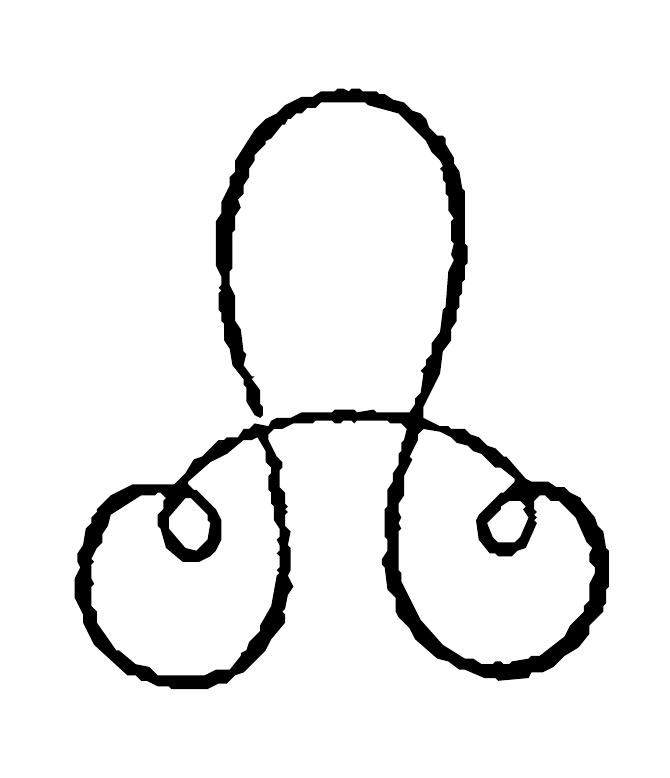
\begin{tikzpicture}[x=1pt,y=-1pt]
\path[use as bounding box] (0,0) rectangle (222,261);
\path[fill=black,draw=none,even odd rule]
(129,24) -- (127,24) -- (126,23) -- (121,23) -- (120,22) -- (117,22) -- (116,23) -- (114,22) -- (112,22) -- (111,23) -- (106,23) -- (103,25) -- (99,25) -- (93,28) -- (90,31) -- (86,33) -- (82,37) -- (75,48) -- (75,52) -- (73,54) -- (73,57) -- (70,63) -- (70,67) -- (68,70) -- (68,86) -- (70,90) -- (70,93) -- (69,94) -- (70,95) -- (69,96) -- (69,102) -- (70,103) -- (70,106) -- (71,107) -- (71,113) -- (73,116) -- (74,122) -- (78,127) -- (78,129) -- (79,130) -- (79,135) -- (82,140) -- (84,141) -- (85,140) -- (85,137) -- (84,136) -- (84,131) -- (81,127) -- (82,126) -- (81,126) -- (78,122) -- (79,118) -- (78,117) -- (77,109) -- (75,106) -- (75,97) -- (73,93) -- (73,88) -- (74,87) -- (74,74) -- (75,73) -- (75,68) -- (77,65) -- (76,62) -- (78,60) -- (78,57) -- (80,54) -- (80,51) -- (82,48) -- (82,46) -- (86,42) -- (86,41) -- (88,40) -- (92,35) -- (93,35) -- (94,33) -- (95,33) -- (97,31) -- (99,31) -- (101,29) -- (104,29) -- (106,27) -- (122,27) -- (123,28) -- (134,31) -- (144,41) -- (146,45) -- (149,48) -- (150,50) -- (149,51) -- (150,52) -- (150,55) -- (151,56) -- (151,60) -- (152,61) -- (152,66) -- (154,69) -- (153,70) -- (153,77) -- (154,78) -- (153,82) -- (154,84) -- (152,88) -- (151,101) -- (150,102) -- (149,110) -- (146,114) -- (146,118) -- (144,120) -- (144,122) -- (142,124) -- (143,125) -- (142,132) -- (140,134) -- (140,136) -- (138,139) -- (126,139) -- (125,138) -- (119,139) -- (118,138) -- (111,138) -- (110,139) -- (99,139) -- (95,141) -- (90,141) -- (88,142) -- (87,144) -- (82,143) -- (80,145) -- (78,145) -- (76,148) -- (72,148) -- (71,149) -- (69,149) -- (63,155) -- (60,156) -- (57,161) -- (53,165) -- (38,165) -- (30,169) -- (25,174) -- (25,175) -- (23,177) -- (23,179) -- (21,181) -- (20,187) -- (18,190) -- (18,193) -- (19,195) -- (17,199) -- (17,206) -- (20,212) -- (20,215) -- (24,223) -- (36,234) -- (39,234) -- (41,236) -- (43,236) -- (47,238) -- (51,238) -- (52,239) -- (65,239) -- (69,237) -- (72,237) -- (75,234) -- (78,233) -- (86,225) -- (88,221) -- (93,215) -- (93,212) -- (92,211) -- (93,210) -- (94,205) -- (96,202) -- (94,198) -- (95,196) -- (95,188) -- (94,187) -- (95,182) -- (93,180) -- (93,176) -- (94,175) -- (93,174) -- (94,173) -- (93,172) -- (93,168) -- (91,166) -- (91,160) -- (92,159) -- (92,157) -- (90,155) -- (87,149) -- (87,147) -- (89,145) -- (92,145) -- (96,143) -- (103,143) -- (104,142) -- (110,142) -- (111,143) -- (113,143) -- (114,142) -- (117,142) -- (118,143) -- (119,142) -- (130,142) -- (131,143) -- (135,143) -- (137,145) -- (136,149) -- (135,150) -- (135,153) -- (134,154) -- (134,158) -- (132,161) -- (132,164) -- (130,167) -- (130,173) -- (129,174) -- (129,184) -- (130,185) -- (130,189) -- (128,192) -- (128,194) -- (129,195) -- (130,203) -- (133,206) -- (133,211) -- (134,213) -- (138,217) -- (140,221) -- (148,228) -- (152,229) -- (156,232) -- (158,232) -- (165,235) -- (169,235) -- (170,236) -- (181,235) -- (182,233) -- (186,233) -- (190,231) -- (194,227) -- (199,224) -- (203,219) -- (203,216) -- (208,211) -- (208,209) -- (209,208) -- (209,203) -- (210,202) -- (210,189) -- (209,188) -- (208,182) -- (206,180) -- (205,177) -- (200,171) -- (200,170) -- (196,168) -- (194,166) -- (191,166) -- (188,164) -- (182,164) -- (180,163) -- (173,155) -- (172,155) -- (169,152) -- (166,151) -- (163,148) -- (160,147) -- (158,145) -- (153,145) -- (152,144) -- (149,144) -- (143,141) -- (143,137) -- (149,125) -- (150,117) -- (153,113) -- (153,109) -- (155,106) -- (155,102) -- (156,101) -- (156,97) -- (157,96) -- (157,92) -- (158,91) -- (158,86) -- (159,85) -- (159,79) -- (158,78) -- (158,59) -- (157,58) -- (156,52) -- (154,49) -- (154,47) -- (151,42) -- (151,40) -- (150,39) -- (148,39) -- (145,36) -- (144,33) -- (142,31) -- (139,30) -- (136,27) -- (132,26) -- cycle
(174,171) -- (178,171) -- (180,173) -- (179,174) -- (181,177) -- (178,184) -- (176,186) -- (170,186) -- (168,184) -- (166,179) -- (171,174) -- (171,173) -- cycle
(57,170) -- (59,170) -- (65,176) -- (65,178) -- (66,179) -- (65,185) -- (61,189) -- (57,188) -- (51,181) -- (51,177) -- cycle
(83,148) -- (86,153) -- (86,157) -- (88,159) -- (88,161) -- (87,162) -- (87,167) -- (88,168) -- (88,172) -- (89,173) -- (89,178) -- (91,181) -- (91,184) -- (90,185) -- (91,187) -- (91,189) -- (90,190) -- (91,191) -- (91,195) -- (90,196) -- (91,197) -- (90,198) -- (88,209) -- (84,216) -- (84,218) -- (80,222) -- (79,225) -- (77,226) -- (77,227) -- (73,232) -- (68,232) -- (64,234) -- (47,234) -- (44,231) -- (39,230) -- (33,225) -- (32,225) -- (25,215) -- (25,211) -- (23,209) -- (23,202) -- (24,201) -- (23,199) -- (23,194) -- (24,193) -- (23,192) -- (25,188) -- (27,186) -- (27,183) -- (29,180) -- (30,176) -- (41,169) -- (46,169) -- (47,168) -- (48,168) -- (50,170) -- (49,171) -- (49,174) -- (47,176) -- (47,180) -- (48,181) -- (50,188) -- (56,193) -- (62,193) -- (66,191) -- (68,189) -- (70,185) -- (70,178) -- (68,174) -- (61,167) -- (60,167) -- (58,165) -- (58,164) -- (66,157) -- (72,154) -- (78,149) -- (81,149) -- cycle
(143,145) -- (149,146) -- (153,148) -- (155,150) -- (159,151) -- (161,153) -- (164,154) -- (169,159) -- (171,159) -- (176,163) -- (176,164) -- (172,168) -- (171,168) -- (163,176) -- (162,178) -- (163,185) -- (167,190) -- (169,190) -- (170,191) -- (175,191) -- (177,189) -- (180,188) -- (184,179) -- (183,178) -- (184,177) -- (183,176) -- (184,175) -- (183,174) -- (183,171) -- (185,169) -- (187,169) -- (189,171) -- (192,171) -- (198,177) -- (202,186) -- (204,188) -- (203,190) -- (203,193) -- (205,195) -- (205,197) -- (203,201) -- (203,207) -- (201,209) -- (201,211) -- (196,216) -- (194,220) -- (185,227) -- (182,227) -- (181,228) -- (175,229) -- (174,230) -- (172,230) -- (171,229) -- (169,229) -- (168,230) -- (164,230) -- (161,228) -- (158,228) -- (150,223) -- (142,214) -- (135,200) -- (135,197) -- (134,196) -- (134,182) -- (135,181) -- (134,179) -- (135,177) -- (134,175) -- (134,172) -- (136,169) -- (136,162) -- (139,156) -- (138,155) -- (141,149) -- (141,147) -- cycle;
\end{tikzpicture}%
}
\hspace{.5em}\resizebox{1.4625cm}{!}{%
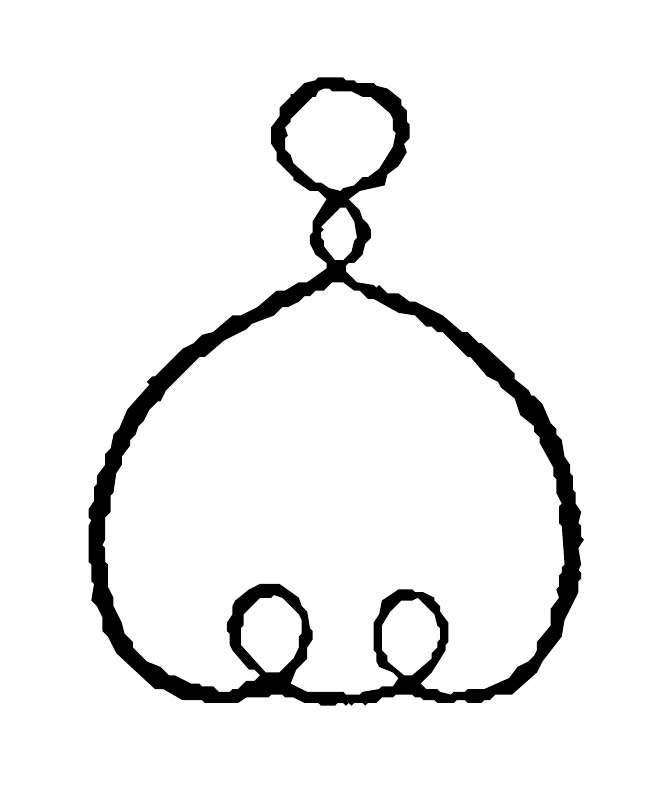
\begin{tikzpicture}[x=1pt,y=-1pt]
\path[use as bounding box] (0,0) rectangle (217,273);
\path[fill=black,draw=none,even odd rule]
(105,18) -- (104,19) -- (100,20) -- (96,24) -- (95,24) -- (95,25) -- (91,29) -- (91,32) -- (88,36) -- (88,42) -- (90,45) -- (90,48) -- (96,54) -- (96,55) -- (102,59) -- (105,59) -- (108,62) -- (103,70) -- (103,74) -- (102,75) -- (102,78) -- (104,82) -- (108,85) -- (108,87) -- (101,92) -- (98,92) -- (93,95) -- (90,95) -- (83,101) -- (77,104) -- (74,104) -- (67,110) -- (63,111) -- (60,114) -- (56,116) -- (46,126) -- (45,126) -- (43,128) -- (44,129) -- (36,138) -- (33,145) -- (31,147) -- (30,152) -- (28,154) -- (28,158) -- (25,162) -- (25,165) -- (24,166) -- (24,171) -- (22,174) -- (22,177) -- (23,178) -- (22,180) -- (22,193) -- (23,194) -- (23,200) -- (24,201) -- (23,207) -- (25,209) -- (27,213) -- (27,218) -- (29,220) -- (32,226) -- (46,239) -- (49,239) -- (56,243) -- (63,243) -- (64,244) -- (76,244) -- (79,242) -- (87,242) -- (88,241) -- (92,241) -- (93,242) -- (96,242) -- (100,244) -- (105,244) -- (106,245) -- (111,245) -- (112,244) -- (114,244) -- (115,245) -- (116,244) -- (117,245) -- (118,244) -- (121,244) -- (122,245) -- (123,244) -- (126,244) -- (128,242) -- (132,242) -- (133,241) -- (139,241) -- (140,242) -- (142,242) -- (143,243) -- (147,243) -- (148,244) -- (154,244) -- (155,243) -- (158,243) -- (159,244) -- (164,244) -- (165,243) -- (167,243) -- (169,241) -- (175,241) -- (184,233) -- (186,229) -- (193,220) -- (194,214) -- (199,204) -- (199,200) -- (200,199) -- (200,197) -- (199,196) -- (200,194) -- (199,188) -- (201,185) -- (200,184) -- (200,180) -- (199,179) -- (200,175) -- (198,172) -- (198,168) -- (197,167) -- (197,162) -- (196,161) -- (196,158) -- (194,155) -- (193,149) -- (191,147) -- (191,145) -- (189,143) -- (186,136) -- (183,133) -- (182,133) -- (181,131) -- (176,127) -- (176,125) -- (164,114) -- (163,114) -- (159,110) -- (157,110) -- (150,104) -- (140,99) -- (138,99) -- (134,96) -- (130,96) -- (127,93) -- (126,94) -- (125,93) -- (119,92) -- (115,88) -- (115,86) -- (116,85) -- (118,85) -- (121,82) -- (122,78) -- (124,76) -- (124,73) -- (123,71) -- (121,69) -- (120,66) -- (116,62) -- (120,59) -- (129,57) -- (130,53) -- (134,50) -- (137,45) -- (136,42) -- (138,40) -- (138,35) -- (137,34) -- (137,30) -- (135,28) -- (135,26) -- (130,22) -- (126,21) -- (125,20) -- (119,20) -- (118,19) -- (115,19) -- (114,18) -- cycle
(141,206) -- (147,212) -- (148,216) -- (149,217) -- (149,221) -- (148,222) -- (148,224) -- (146,226) -- (146,228) -- (139,234) -- (136,234) -- (130,229) -- (130,227) -- (128,225) -- (128,216) -- (131,211) -- (135,207) -- (139,207) -- cycle
(89,205) -- (92,206) -- (98,212) -- (99,214) -- (99,219) -- (98,220) -- (98,224) -- (96,228) -- (91,233) -- (86,233) -- (77,223) -- (77,217) -- (78,216) -- (78,212) -- (84,206) -- (88,206) -- cycle
(62,119) -- (64,119) -- (71,113) -- (79,109) -- (81,107) -- (89,104) -- (92,101) -- (94,101) -- (98,99) -- (100,97) -- (102,97) -- (104,95) -- (107,95) -- (110,92) -- (114,92) -- (118,95) -- (120,95) -- (123,98) -- (125,98) -- (134,103) -- (140,104) -- (144,108) -- (146,108) -- (148,110) -- (150,110) -- (159,119) -- (160,119) -- (166,126) -- (170,128) -- (171,130) -- (176,134) -- (178,140) -- (183,144) -- (183,146) -- (185,148) -- (185,150) -- (190,159) -- (190,162) -- (191,163) -- (191,168) -- (193,172) -- (192,173) -- (192,179) -- (193,180) -- (194,194) -- (193,195) -- (193,197) -- (192,198) -- (192,202) -- (191,203) -- (192,206) -- (189,210) -- (189,216) -- (184,222) -- (184,225) -- (183,227) -- (181,229) -- (177,231) -- (174,235) -- (165,239) -- (159,239) -- (158,240) -- (154,240) -- (153,241) -- (149,240) -- (148,239) -- (144,239) -- (142,237) -- (146,233) -- (151,225) -- (151,223) -- (152,222) -- (152,215) -- (149,211) -- (149,209) -- (147,207) -- (147,206) -- (143,204) -- (140,204) -- (139,203) -- (134,203) -- (128,207) -- (127,212) -- (125,215) -- (125,225) -- (126,226) -- (126,229) -- (127,231) -- (132,233) -- (134,235) -- (132,238) -- (128,238) -- (127,239) -- (121,240) -- (120,241) -- (115,241) -- (114,240) -- (101,240) -- (95,237) -- (97,232) -- (101,228) -- (101,224) -- (103,221) -- (103,218) -- (102,217) -- (101,211) -- (99,209) -- (98,206) -- (91,201) -- (84,201) -- (80,203) -- (75,207) -- (74,209) -- (74,212) -- (72,215) -- (72,218) -- (73,219) -- (73,223) -- (74,225) -- (80,232) -- (82,232) -- (84,234) -- (82,236) -- (79,236) -- (76,239) -- (74,239) -- (73,240) -- (69,240) -- (67,238) -- (63,238) -- (62,237) -- (59,237) -- (53,234) -- (51,234) -- (48,231) -- (43,229) -- (38,224) -- (38,222) -- (35,219) -- (34,215) -- (31,209) -- (31,206) -- (29,202) -- (29,194) -- (28,193) -- (28,188) -- (27,187) -- (28,185) -- (28,177) -- (30,175) -- (30,169) -- (31,168) -- (32,161) -- (34,158) -- (34,155) -- (37,151) -- (37,149) -- (39,147) -- (40,144) -- (42,142) -- (44,138) -- (47,135) -- (48,135) -- (50,131) -- cycle
(115,65) -- (118,70) -- (119,76) -- (118,77) -- (117,81) -- (114,84) -- (111,84) -- (107,79) -- (107,77) -- (106,76) -- (106,74) -- (107,73) -- (106,72) -- (113,65) -- cycle
(107,22) -- (109,22) -- (110,23) -- (117,23) -- (121,25) -- (124,25) -- (131,31) -- (132,33) -- (132,37) -- (133,38) -- (132,43) -- (127,51) -- (123,54) -- (121,54) -- (118,57) -- (114,58) -- (113,59) -- (109,58) -- (106,56) -- (104,56) -- (96,49) -- (95,46) -- (93,44) -- (93,40) -- (94,39) -- (93,36) -- (95,34) -- (95,33) -- (103,25) -- (104,25) -- (105,23) -- cycle;
\end{tikzpicture}%
}
\hspace{.5em}\resizebox{1.575cm}{!}{%
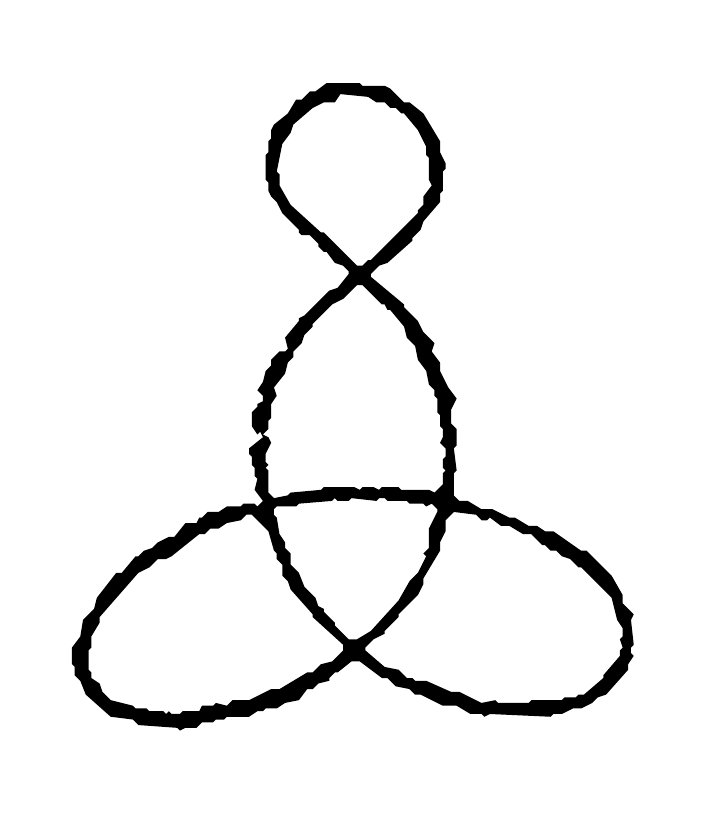
\begin{tikzpicture}[x=1pt,y=-1pt]
\path[use as bounding box] (0,0) rectangle (233,278);
\path[fill=black,draw=none,even odd rule]
(108,20) -- (104,23) -- (102,23) -- (99,26) -- (97,26) -- (94,31) -- (89,35) -- (88,37) -- (88,40) -- (87,41) -- (87,45) -- (86,46) -- (86,55) -- (87,56) -- (87,59) -- (88,61) -- (90,63) -- (92,67) -- (98,73) -- (98,74) -- (99,75) -- (102,75) -- (105,78) -- (105,79) -- (107,81) -- (108,81) -- (111,85) -- (114,86) -- (116,88) -- (116,89) -- (112,94) -- (109,95) -- (100,104) -- (98,105) -- (98,106) -- (93,112) -- (94,116) -- (93,117) -- (91,117) -- (88,120) -- (88,122) -- (86,124) -- (85,128) -- (83,131) -- (85,133) -- (85,135) -- (83,136) -- (83,137) -- (81,139) -- (81,144) -- (83,147) -- (84,146) -- (85,148) -- (80,152) -- (80,154) -- (81,155) -- (81,158) -- (82,159) -- (82,162) -- (83,163) -- (82,167) -- (85,171) -- (83,173) -- (82,172) -- (78,172) -- (77,173) -- (72,173) -- (69,175) -- (65,175) -- (63,177) -- (62,177) -- (61,179) -- (57,179) -- (53,184) -- (51,184) -- (47,186) -- (45,188) -- (42,189) -- (40,191) -- (39,191) -- (34,197) -- (32,197) -- (25,206) -- (24,210) -- (20,214) -- (19,220) -- (16,224) -- (16,230) -- (17,231) -- (17,234) -- (19,236) -- (21,241) -- (30,249) -- (38,250) -- (40,252) -- (54,253) -- (55,254) -- (57,253) -- (61,253) -- (63,251) -- (67,251) -- (68,250) -- (71,250) -- (72,249) -- (80,249) -- (83,247) -- (85,247) -- (86,246) -- (90,246) -- (93,244) -- (98,243) -- (101,239) -- (103,239) -- (105,237) -- (109,236) -- (109,235) -- (111,233) -- (112,233) -- (117,229) -- (120,229) -- (128,235) -- (130,235) -- (133,238) -- (138,239) -- (140,241) -- (142,241) -- (150,245) -- (155,245) -- (160,248) -- (164,248) -- (165,249) -- (167,248) -- (189,249) -- (190,248) -- (193,248) -- (197,246) -- (200,246) -- (204,244) -- (206,242) -- (209,241) -- (217,232) -- (217,230) -- (219,227) -- (218,226) -- (218,224) -- (219,223) -- (218,214) -- (219,212) -- (215,208) -- (215,205) -- (211,198) -- (202,189) -- (200,189) -- (190,182) -- (187,182) -- (184,180) -- (181,180) -- (176,177) -- (174,177) -- (168,174) -- (164,174) -- (159,171) -- (156,171) -- (154,169) -- (154,161) -- (155,160) -- (154,152) -- (155,151) -- (155,145) -- (153,143) -- (153,138) -- (155,134) -- (152,130) -- (149,124) -- (149,121) -- (146,117) -- (147,114) -- (143,110) -- (141,106) -- (136,101) -- (136,100) -- (124,90) -- (124,89) -- (127,86) -- (130,85) -- (139,77) -- (139,76) -- (142,73) -- (143,70) -- (149,63) -- (149,60) -- (150,59) -- (150,52) -- (151,51) -- (151,49) -- (149,45) -- (149,41) -- (143,31) -- (138,27) -- (136,27) -- (131,22) -- (129,21) -- (121,21) -- (120,20) -- cycle
(114,223) -- (114,225) -- (110,229) -- (106,230) -- (103,233) -- (101,233) -- (91,239) -- (88,239) -- (80,243) -- (74,243) -- (72,245) -- (68,244) -- (67,245) -- (63,245) -- (62,247) -- (56,247) -- (55,248) -- (52,248) -- (51,247) -- (50,248) -- (49,247) -- (44,247) -- (43,246) -- (39,246) -- (38,245) -- (30,243) -- (27,240) -- (26,237) -- (23,235) -- (23,233) -- (22,232) -- (22,225) -- (23,224) -- (23,220) -- (26,215) -- (26,213) -- (40,197) -- (44,195) -- (47,192) -- (50,192) -- (52,191) -- (62,183) -- (64,183) -- (66,181) -- (69,181) -- (72,179) -- (77,178) -- (79,176) -- (81,176) -- (87,182) -- (89,189) -- (90,190) -- (90,192) -- (92,194) -- (92,198) -- (94,200) -- (95,203) -- (103,212) -- (103,213) -- cycle
(154,175) -- (162,176) -- (164,178) -- (166,178) -- (167,177) -- (171,180) -- (174,180) -- (179,183) -- (182,183) -- (186,187) -- (187,187) -- (189,189) -- (191,189) -- (193,191) -- (196,192) -- (199,195) -- (200,195) -- (211,206) -- (213,214) -- (215,217) -- (215,220) -- (214,221) -- (215,224) -- (214,225) -- (214,227) -- (208,234) -- (208,235) -- (201,241) -- (199,241) -- (198,242) -- (194,242) -- (193,243) -- (182,243) -- (181,244) -- (170,244) -- (169,243) -- (164,244) -- (156,240) -- (153,240) -- (144,236) -- (140,236) -- (139,235) -- (137,235) -- (134,232) -- (129,231) -- (122,225) -- (122,224) -- (125,221) -- (129,219) -- (129,218) -- (134,213) -- (134,212) -- (141,205) -- (143,201) -- (143,199) -- (149,189) -- (149,186) -- (151,182) -- (151,178) -- cycle
(90,173) -- (97,173) -- (98,172) -- (110,171) -- (111,170) -- (112,171) -- (116,171) -- (117,170) -- (126,171) -- (127,170) -- (129,170) -- (130,171) -- (137,171) -- (138,172) -- (143,172) -- (144,173) -- (146,172) -- (148,174) -- (148,175) -- (145,181) -- (145,188) -- (143,190) -- (144,191) -- (141,197) -- (138,200) -- (134,207) -- (124,218) -- (119,221) -- (116,221) -- (111,216) -- (111,215) -- (107,211) -- (107,210) -- (105,209) -- (104,206) -- (100,202) -- (98,197) -- (95,194) -- (95,190) -- (93,188) -- (93,186) -- (91,183) -- (90,177) -- (89,176) -- (89,174) -- cycle
(121,93) -- (128,100) -- (129,100) -- (130,102) -- (131,102) -- (136,108) -- (137,112) -- (140,115) -- (141,120) -- (144,124) -- (145,129) -- (147,131) -- (147,133) -- (148,134) -- (148,139) -- (149,140) -- (149,144) -- (150,145) -- (150,148) -- (149,150) -- (151,152) -- (151,155) -- (150,156) -- (150,159) -- (151,160) -- (150,161) -- (150,165) -- (147,168) -- (145,167) -- (135,167) -- (134,166) -- (128,166) -- (127,167) -- (125,166) -- (121,166) -- (120,167) -- (118,166) -- (107,166) -- (106,167) -- (95,168) -- (94,169) -- (89,170) -- (87,168) -- (87,160) -- (86,159) -- (87,158) -- (86,157) -- (86,154) -- (88,150) -- (87,148) -- (85,147) -- (87,145) -- (87,142) -- (88,141) -- (88,136) -- (90,133) -- (89,130) -- (93,125) -- (94,121) -- (96,119) -- (96,117) -- (99,114) -- (100,111) -- (103,108) -- (103,107) -- (110,100) -- (114,98) -- (119,93) -- cycle
(113,24) -- (123,25) -- (126,27) -- (129,27) -- (131,29) -- (133,29) -- (135,31) -- (136,31) -- (141,37) -- (144,43) -- (144,46) -- (145,47) -- (145,55) -- (146,57) -- (143,61) -- (143,64) -- (141,66) -- (141,67) -- (124,84) -- (123,84) -- (121,86) -- (119,86) -- (107,74) -- (106,74) -- (95,64) -- (91,57) -- (91,53) -- (90,52) -- (92,42) -- (95,38) -- (96,35) -- (103,29) -- (107,27) -- (111,27) -- cycle;
\end{tikzpicture}%
}

\par\medskip\resizebox{1.6875cm}{!}{%
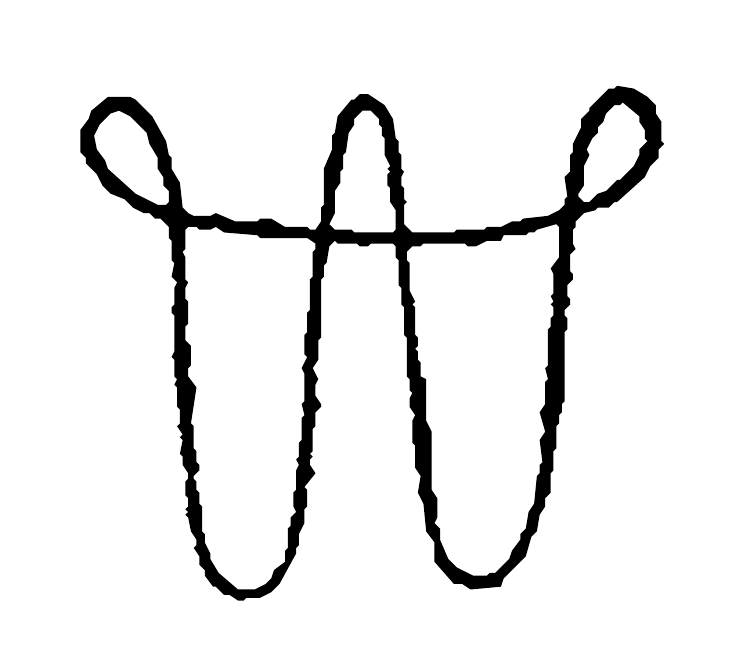
\begin{tikzpicture}[x=1pt,y=-1pt]
\path[use as bounding box] (0,0) rectangle (250,222);
\path[fill=black,draw=none,even odd rule]
(224,25) -- (219,22) -- (213,21) -- (212,22) -- (210,22) -- (203,29) -- (203,30) -- (200,33) -- (200,36) -- (197,42) -- (197,45) -- (196,46) -- (196,52) -- (194,54) -- (195,61) -- (194,62) -- (194,64) -- (192,66) -- (188,68) -- (179,69) -- (178,70) -- (175,70) -- (171,72) -- (166,72) -- (165,73) -- (155,73) -- (154,74) -- (139,74) -- (136,71) -- (136,64) -- (137,63) -- (136,62) -- (136,58) -- (135,57) -- (135,54) -- (136,52) -- (135,51) -- (135,46) -- (134,45) -- (134,41) -- (133,40) -- (132,33) -- (129,28) -- (123,24) -- (120,24) -- (118,26) -- (117,26) -- (112,32) -- (111,38) -- (110,39) -- (110,44) -- (107,51) -- (107,64) -- (106,65) -- (106,70) -- (104,73) -- (102,73) -- (101,72) -- (93,72) -- (88,69) -- (84,69) -- (83,70) -- (75,70) -- (68,67) -- (66,68) -- (60,68) -- (58,67) -- (56,65) -- (55,56) -- (52,51) -- (52,47) -- (51,46) -- (50,41) -- (45,32) -- (39,26) -- (37,25) -- (29,25) -- (23,30) -- (22,33) -- (19,37) -- (19,45) -- (21,47) -- (21,49) -- (25,53) -- (27,57) -- (30,60) -- (35,62) -- (38,65) -- (42,67) -- (44,67) -- (46,69) -- (48,69) -- (51,72) -- (51,76) -- (52,77) -- (52,84) -- (53,85) -- (52,90) -- (54,92) -- (53,94) -- (53,100) -- (52,101) -- (52,103) -- (53,104) -- (53,117) -- (52,119) -- (53,120) -- (53,126) -- (54,127) -- (53,129) -- (54,130) -- (54,137) -- (55,138) -- (55,143) -- (54,144) -- (56,147) -- (55,148) -- (56,149) -- (55,154) -- (56,155) -- (56,158) -- (58,161) -- (58,163) -- (57,164) -- (57,169) -- (58,170) -- (58,173) -- (57,174) -- (58,175) -- (57,176) -- (58,177) -- (59,182) -- (61,185) -- (61,187) -- (60,188) -- (62,191) -- (62,194) -- (64,196) -- (64,198) -- (67,202) -- (68,202) -- (71,205) -- (73,205) -- (76,207) -- (78,207) -- (79,206) -- (84,206) -- (88,204) -- (91,201) -- (97,190) -- (97,188) -- (98,187) -- (98,183) -- (100,179) -- (100,174) -- (101,173) -- (101,167) -- (100,166) -- (104,161) -- (102,158) -- (102,156) -- (103,155) -- (102,154) -- (103,153) -- (103,145) -- (104,144) -- (104,139) -- (106,137) -- (106,136) -- (104,133) -- (104,129) -- (105,127) -- (103,123) -- (105,120) -- (105,113) -- (106,112) -- (106,91) -- (107,90) -- (107,86) -- (108,85) -- (109,79) -- (111,77) -- (112,78) -- (119,78) -- (120,79) -- (123,79) -- (124,78) -- (132,78) -- (133,79) -- (133,83) -- (134,84) -- (134,93) -- (135,94) -- (135,100) -- (136,101) -- (136,111) -- (137,112) -- (137,126) -- (138,127) -- (138,131) -- (139,132) -- (138,134) -- (138,137) -- (140,140) -- (139,142) -- (139,150) -- (140,151) -- (140,159) -- (142,162) -- (141,168) -- (143,172) -- (144,182) -- (147,186) -- (147,193) -- (154,201) -- (157,201) -- (160,203) -- (171,202) -- (172,199) -- (180,191) -- (182,184) -- (184,182) -- (185,176) -- (187,173) -- (187,170) -- (189,168) -- (189,161) -- (190,160) -- (190,153) -- (191,152) -- (191,144) -- (192,143) -- (192,140) -- (193,139) -- (193,136) -- (194,135) -- (194,110) -- (195,109) -- (195,105) -- (194,104) -- (194,102) -- (196,100) -- (196,98) -- (195,97) -- (195,93) -- (197,91) -- (197,89) -- (196,88) -- (196,82) -- (198,80) -- (197,78) -- (197,73) -- (198,72) -- (198,70) -- (201,67) -- (205,66) -- (206,65) -- (210,65) -- (212,63) -- (213,63) -- (223,54) -- (225,50) -- (228,47) -- (228,44) -- (230,42) -- (229,41) -- (229,34) -- (227,31) -- (227,28) -- cycle
(58,72) -- (61,72) -- (62,73) -- (66,73) -- (68,72) -- (71,74) -- (83,75) -- (84,76) -- (101,76) -- (104,78) -- (104,80) -- (103,81) -- (103,90) -- (102,91) -- (102,102) -- (101,103) -- (101,110) -- (100,111) -- (100,118) -- (101,119) -- (99,123) -- (100,125) -- (100,135) -- (99,136) -- (100,140) -- (99,141) -- (99,149) -- (98,150) -- (98,155) -- (97,156) -- (98,158) -- (97,160) -- (97,167) -- (96,168) -- (96,173) -- (97,175) -- (95,177) -- (95,180) -- (94,181) -- (94,188) -- (93,189) -- (93,193) -- (89,196) -- (88,199) -- (86,201) -- (82,203) -- (76,203) -- (69,197) -- (66,192) -- (66,190) -- (64,186) -- (64,183) -- (63,182) -- (63,173) -- (62,172) -- (62,168) -- (61,167) -- (61,164) -- (60,163) -- (60,162) -- (62,160) -- (62,158) -- (61,157) -- (61,153) -- (60,152) -- (60,144) -- (59,143) -- (61,130) -- (58,126) -- (58,123) -- (59,122) -- (59,115) -- (57,113) -- (57,108) -- (58,107) -- (58,99) -- (57,98) -- (57,94) -- (58,92) -- (57,91) -- (57,83) -- (56,81) -- (57,80) -- (57,73) -- cycle
(191,71) -- (192,72) -- (192,83) -- (189,87) -- (190,89) -- (190,96) -- (189,97) -- (190,99) -- (189,100) -- (190,101) -- (190,104) -- (189,105) -- (189,108) -- (188,109) -- (188,122) -- (187,123) -- (188,127) -- (187,128) -- (187,136) -- (185,139) -- (187,146) -- (185,149) -- (186,157) -- (185,158) -- (185,161) -- (184,162) -- (183,172) -- (181,175) -- (180,181) -- (178,183) -- (178,185) -- (175,189) -- (174,192) -- (169,197) -- (167,197) -- (166,198) -- (161,198) -- (155,195) -- (152,192) -- (149,185) -- (149,181) -- (147,179) -- (148,177) -- (148,170) -- (146,167) -- (146,146) -- (144,142) -- (144,127) -- (142,126) -- (142,121) -- (141,120) -- (141,117) -- (140,116) -- (141,115) -- (141,112) -- (140,111) -- (140,101) -- (139,100) -- (140,99) -- (138,95) -- (138,85) -- (137,84) -- (137,81) -- (139,79) -- (142,79) -- (143,78) -- (158,78) -- (159,79) -- (162,79) -- (166,77) -- (171,77) -- (172,75) -- (180,75) -- (181,74) -- (183,74) -- (184,73) -- cycle
(121,30) -- (124,30) -- (127,33) -- (127,35) -- (128,36) -- (128,39) -- (129,40) -- (129,46) -- (131,50) -- (130,51) -- (131,52) -- (130,53) -- (130,57) -- (131,58) -- (131,63) -- (133,66) -- (133,73) -- (132,74) -- (118,74) -- (117,73) -- (111,73) -- (109,71) -- (111,67) -- (111,59) -- (113,56) -- (113,52) -- (114,51) -- (114,46) -- (115,45) -- (116,38) -- (118,35) -- (118,33) -- cycle
(30,31) -- (33,30) -- (37,32) -- (43,38) -- (44,42) -- (47,47) -- (47,51) -- (49,54) -- (49,57) -- (51,59) -- (51,63) -- (50,64) -- (47,64) -- (39,60) -- (29,51) -- (28,48) -- (25,44) -- (24,39) -- (26,35) -- cycle
(215,27) -- (221,32) -- (221,34) -- (223,37) -- (223,40) -- (224,41) -- (221,44) -- (221,46) -- (219,50) -- (214,55) -- (213,55) -- (209,59) -- (206,60) -- (203,63) -- (201,63) -- (199,61) -- (199,60) -- (201,57) -- (201,50) -- (203,46) -- (202,44) -- (204,40) -- (206,38) -- (206,36) -- (208,34) -- (209,31) -- (212,28) -- (214,28) -- cycle;
\end{tikzpicture}%
}

\end{center}

Sehr vereinfacht wird die Registrirung, indem man die Plätze mit 0, 1, 2,
3 u.\,s.\,w.\ bezeichnet, und diejenigen Paare von Plätzen, die Einem Knoten
entsprechen, neben einander setzt. In einem möglichen geschlossenen Tracte
muss jedes Paar aus einer geraden und einer ungeraden Zahl bestehen. Z.\,B.

\begin{center}
Nr.\ 91 $\left|\begin{array}{c}0.7\\2.5\\4.1\\6.3\end{array}\right\|$
\quad Nr.\ 48 $\left|\begin{array}{c}0.3\\2.7\\4.1\\6.5\end{array}\right|$
u.\,s.\,w.
\end{center}

Dieses Criterium hört aber bei Perioden von mehr als 4 Knoten auf, für
die Möglichkeit zureichend zu sein; z.\,B. \emph{abcadcedbe} oder
$\left(\begin{array}{ccccc}0. & 2. & 4. & 6. & 8 \\ 3. & 5. & 7. & 9. & 1\end{array}\right)$
ist, obgleich dem Criterium genügt ist, unmöglich.

Ebenso ist unmöglich \emph{abcabdecde} [oder]
$\left(\begin{array}{ccccc}0. & 2. & 4. & 6. & 8 \\ 3. & 7. & 1. & 9. & 5\end{array}\right)$.

Die vollständige lexicographische Aufzählung aller 120 Tractcombinationen
für 5 Knoten auf der folgenden Seite [, wobei die unmöglichen Tracte durch
einen Stern bezeichnet sind.]
